%=====================================================================
%  Transparent USB Storage Passthrough across Same-Host Live Migration
%  with a Multi-Client vfio-user Backend
%
%  Build:  make        (or: latexmk -pdf main.tex)
%=====================================================================
\documentclass[10pt,conference]{IEEEtran}

\usepackage[T1]{fontenc}
\usepackage[utf8]{inputenc}
\usepackage{cite}
\usepackage{amsmath,amssymb}
\usepackage{graphicx}
\usepackage{booktabs}
\usepackage{array}
\usepackage{url}
\usepackage{tikz}
\usepackage{pgfplots}
\usetikzlibrary{positioning,arrows.meta,decorations.pathreplacing,calc}
\pgfplotsset{compat=1.18}
\usepackage[hidelinks]{hyperref}

\newcommand{\code}[1]{\texttt{#1}}

\title{Transparent USB Storage Passthrough across Same-Host\\
Virtual Machine Live Migration with a Multi-Client\\
vfio-user Backend}

\author{\IEEEauthorblockN{Author Name}
\IEEEauthorblockA{Department, University\\
Email: author@example.edu}
\and
\IEEEauthorblockN{Supervisor Name}
\IEEEauthorblockA{Department, University\\
Email: supervisor@example.edu}
}

\begin{document}
\maketitle

\begin{abstract}
Passing a physical USB device through to a virtual machine is attractive for
storage, dongles and instrumentation, but it collides with live migration:
the host-side device session (open file descriptors, claimed interfaces,
endpoint state and the device's internal state) cannot be serialised, so any
migration path that tears the session down forces the guest to re-enumerate.
This paper studies the concrete case of Cloud Hypervisor together with
\code{usbvfiod}, a Rust vfio-user server that emulates an xHCI controller. We
first show, by measurement, that migrating a VM with a vfio-user device
\emph{deadlocks}: the destination blocks for $199.9$\,s inside the protocol
version handshake because the vfio-user server accepts exactly one connection,
which the source still owns. We then present a design that removes the
deadlock without changing the VMM: because the vfio-user handshake commands
never touch the device backend, a wrapper that takes the backend lock
\emph{per command} rather than per connection lets a second client connect
while the first is still attached. We identify and fix two further defects that
the hand-over exposes---a departing client tearing down the surviving client's
interrupt line and DMA mappings, and completion interrupts lost inside the
hand-over window---and we describe a measurement harness that reads the
verdict from the guest's own log rather than from host-side observation.
On a real 32\,GB exfat stick passed through to an Ubuntu 22.04 guest, a
128\,MiB file copy that spans the migration completes in 10 out of 10 runs
with a measured downtime of 4--18\,ms, byte-identical data and zero
re-enumeration, resets or I/O errors in the guest.
\end{abstract}

\begin{IEEEkeywords}
virtualisation, live migration, device passthrough, vfio-user, USB, xHCI,
Cloud Hypervisor, KVM
\end{IEEEkeywords}

%=====================================================================
\section{Introduction}
%=====================================================================

Virtual machines are routinely equipped with physical devices through
passthrough so that they can use hardware that is either impossible or
unattractive to emulate. Live migration---moving a running VM between VMM
instances with a downtime short enough to be unnoticeable---is the standard
mechanism for host maintenance, load balancing and upgrades
\cite{clark2005live}. The two techniques, however, interact badly.

Memory and CPU state migrate well, and kernel VFIO devices can migrate when
the device implements the VFIO migration interface \cite{kernelvfio}. USB
devices are the difficult case. A guest talks to a USB device through a host
controller; a passthrough implementation either emulates that controller and
forwards individual transfers, or hands the whole controller to the guest. In
the first case the host process that owns the physical device holds a session
that is \emph{not} part of the guest state: an open file descriptor, a claimed
interface, endpoint configuration and, above all, the device's own internal
state. None of this can be serialised. Any migration that recreates the device
on the destination therefore forces the guest to observe a disconnect and a
re-enumeration, which at minimum interrupts I/O and can invalidate host-side
state such as a mounted filesystem or an encrypted volume.

Cloud Hypervisor (CH) supports USB passthrough through the vfio-user protocol
via \code{-{}-user-device socket=...} \cite{chvfiouser}. The server side can be
\code{usbvfiod} \cite{usbvfiodrepo}, which emulates an xHCI controller and
forwards transfers to the physical device with \code{nusb} \cite{nusb}. CH
documents live migration \cite{chlive}, but the vfio-user path was never
exercised under migration.

This paper starts from a measurement: migrating a CH VM that has a vfio-user
device attached does not fail cleanly---it \emph{hangs}, and it hangs on the
destination VMM (Section~\ref{sec:problem}). We then design and implement a
solution that makes a same-host migration of such a VM work, and we measure it
end to end with real hardware.

\subsection{Contributions}
\begin{enumerate}
  \item We characterise, by measurement and source inspection, why a
        vfio-user device deadlocks a CH live migration: the destination VMM
        blocks in the version handshake because the server accepts a single
        connection that the source still holds. We quantify it (199.9\,s of
        zero progress; the destination never gets a reply) and show that even a
        successful takeover would not transfer device state
        (Section~\ref{sec:problem}).
  \item We present a \emph{multi-client} vfio-user backend design that removes
        the deadlock without modifying the VMM. The key observation is that the
        handshake commands never reach the device backend, so the backend lock
        can be taken per command instead of per connection
        (Section~\ref{sec:design}).
  \item We identify and fix two defects that only appear once a hand-over is
        possible: a departing client disabling the surviving client's interrupt
        line and unmapping its DMA regions, and completion interrupts being
        delivered to the departing VMM's event descriptor inside the
        hand-over window (Sections~\ref{sec:ownership}
        and~\ref{sec:interrupt}).
  \item We build a reproducible end-to-end harness, including a guest image
        and a measurement method whose verdict is read from the \emph{guest's
        own log} rather than from host-side observation, and we report the
        design decisions that this method forced us to change
        (Section~\ref{sec:implementation}).
  \item We evaluate the result with a real USB stick: 10 out of 10 migrations
        of a VM that is copying a 128\,MiB file at the time of the migration
        succeed with 4--18\,ms downtime, byte-identical data and no
        re-enumeration or reset in the guest (Section~\ref{sec:evaluation}).
\end{enumerate}

\subsection{Paper organisation}
Section~\ref{sec:background} reviews live migration, device passthrough and
USB passthrough alternatives.  Section~\ref{sec:problem} analyses the measured
deadlock. Section~\ref{sec:design} presents the design,
Section~\ref{sec:implementation} the implementation.
Section~\ref{sec:evaluation} evaluates, Section~\ref{sec:discussion} discusses
limitations, and Section~\ref{sec:conclusion} concludes.

%=====================================================================
\section{Background and Related Work}
\label{sec:background}
%=====================================================================

\subsection{Live migration}
Live migration of VMs was popularised by Clark \emph{et al.}
\cite{clark2005live}, who introduced pre-copy migration: pages are copied
while the VM runs, and a final stop-and-copy phase transfers the remaining
dirty pages while the VM is paused. KVM \cite{kivity2007kvm} made this a
mainstream kernel mechanism, and modern VMMs such as Firecracker
\cite{agache2020firecracker} and Cloud Hypervisor \cite{chrepo} implement
variants of it. Cloud Hypervisor documents both TCP and UNIX-socket transports;
for same-host migration it offers \code{memory\_mode=memfds}, which passes the
guest memory \emph{backing file descriptors} over the socket so that source and
destination map the same memory instead of copying it \cite{chlive}. This is
the mode we use: it makes the memory identical in both VMMs, which is what
allows a vfio-user server on the host to keep its DMA mappings.

\subsection{Device passthrough: VFIO and vfio-user}
VFIO is the Linux framework that exposes a device to user space with an
IOMMU-backed DMA model \cite{kernelvfio}. In the kernel-VFIO model the VMM maps
device BARs and registers event descriptors directly. vfio-user moves the same
programming model to a user-space server reached over a UNIX socket
\cite{qemuvfiouser}: a client (the VMM) queries regions, reads and writes
device memory, maps guest memory for device DMA, registers interrupt file
descriptors, and may reset the device. The protocol specification is maintained
with QEMU \cite{qemuvfiouser} and reference implementations exist in
\code{libvfio-user} \cite{libvfiouser}. Cloud Hypervisor implements the client
side \cite{chvfiouser}; the \code{vfio\_user} crate \cite{vfiousercrate}, part
of the rust-vmm collection \cite{rustvmmvfio}, implements both sides and is
used by CH and by \code{usbvfiod}.

\subsection{USB passthrough alternatives}
Table~\ref{tab:approaches} compares the options we considered. Passing through
with a user-space server over vfio-user is the approach of \code{usbvfiod} and
the subject of this paper: it keeps the guest driver unmodified and confines
the device to an unprivileged process, at the cost of an emulated controller in
the transfer path. USB/IP \cite{hirofuchi2005usbip,kernelusbip} tunnels USB
traffic over a network and is the natural answer for \emph{cross-host} device
sharing, but the device remains attached to the source host and depends on an
external transport. QEMU's USB redirection \cite{qemuusb} and the virtio
specification \cite{virtio12} provide guest-side USB stacks whose transport can
in principle be made migratable, but they require a guest driver and do not
preserve a host-side session across a migration on their own.

\begin{table}[t]
\centering
\caption{USB passthrough approaches.}
\label{tab:approaches}
\footnotesize
\setlength{\tabcolsep}{3pt}
\begin{tabular}{@{}p{1.5cm}p{2.5cm}p{3.0cm}@{}}
\toprule
Approach & Where device state lives & Consequence for migration \\
\midrule
Kernel USB driver in guest (\code{usbfs} in host process) & host process, not serialisable & session must survive; used here \\
USB/IP \cite{hirofuchi2005usbip} & source host, exported over network & source must stay online; transport in path \\
QEMU USB redirection \cite{qemuusb} & emulated device in VMM & re-created on destination \\
virtio-usb \cite{virtio12} & paravirtual, guest driver & guest-visible change; driver required \\
\bottomrule
\end{tabular}
\end{table}

\subsection{Emulated xHCI and USB mass storage}
\code{usbvfiod} presents an xHCI controller \cite{xhcispec} to the guest. The
Linux xHCI driver discovers the controller, performs a host controller reset,
enumerates the attached devices and then drives transfers through command,
event and transfer rings in guest memory. Mass-storage devices use the
Bulk-Only Transport protocol \cite{usbbot}, which the kernel's
\code{usb-storage} module implements. Our measurements use this path because it
is the most common passthrough workload and because a bulk transfer makes the
consequences of a lost completion immediately visible as an I/O error.

Fig.~\ref{fig:arch} summarises the resulting architecture. The physical device
is owned by a host process for the entire lifetime of the VM, including the
migration; the VMM is only a client of that process, and the guest sees an
ordinary controller.

\begin{figure*}[t]
\centering
% Figure: system architecture.
% Chain: physical USB stick -> usbvfiod -> vfio-user -> Cloud Hypervisor -> guest.
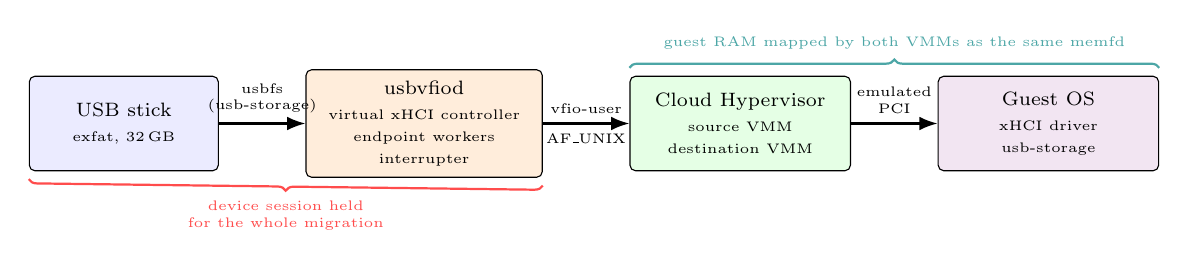
\begin{tikzpicture}[
  font=\scriptsize,
  >=Latex,
  node distance=11mm,
  blk/.style={draw, rounded corners=2pt, align=center, inner sep=4pt,
              minimum height=12mm, minimum width=24mm},
  ar/.style={->, thick},
]
  \node[blk, fill=blue!8] (dev) {USB stick\\[1pt]\tiny exfat, 32\,GB};
  \node[blk, fill=orange!14, right=of dev, minimum width=30mm] (uvf)
        {usbvfiod\\[1pt]\tiny virtual xHCI controller\\\tiny endpoint workers\\\tiny interrupter};
  \node[blk, fill=green!10, right=of uvf, minimum width=28mm] (ch)
        {Cloud Hypervisor\\[1pt]\tiny source VMM\\\tiny destination VMM};
  \node[blk, fill=violet!10, right=of ch, minimum width=28mm] (g)
        {Guest OS\\[1pt]\tiny xHCI driver\\\tiny usb-storage};

  \draw[ar] (dev) -- node[above, font=\tiny, align=center]{usbfs\\(usb-storage)} (uvf);
  \draw[ar] (uvf) -- node[above, font=\tiny]{vfio-user} node[below, font=\tiny]{AF\_UNIX} (ch);
  \draw[ar] (ch) -- node[above, font=\tiny, align=center]{emulated\\PCI} (g);

  % annotations
  \draw[decorate, decoration={brace, amplitude=3pt, mirror}, thick, red!70]
        ([yshift=-1mm]dev.south west) -- ([yshift=-1mm]uvf.south east)
        node[midway, below=3pt, font=\tiny, align=center, red!70]
        {device session held\\for the whole migration};
  \draw[decorate, decoration={brace, amplitude=3pt}, thick, teal!70]
        ([yshift=1mm]ch.north west) -- ([yshift=1mm]g.north east)
        node[midway, above=3pt, font=\tiny, align=center, teal!70]
        {guest RAM mapped by both VMMs as the same memfd};
\end{tikzpicture}

\caption{System architecture. \code{usbvfiod} owns the physical USB device and
emulates an xHCI controller; the VMM reaches it over vfio-user. During a
same-host migration the server process is never restarted, so the device
session and the controller state survive, and both VMMs map the same guest
memory.}
\label{fig:arch}
\end{figure*}

%=====================================================================
\section{Problem Analysis}
\label{sec:problem}
%=====================================================================

\subsection{Experimental setup}
All measurements were taken on a single host running Debian~13 with Linux
6.17.4, 8 cores and 62\,GiB of RAM, on which the KVM module is loaded
\cite{kivity2007kvm}. Table~\ref{tab:setup} lists the software under test. The
guest is Ubuntu 22.04.4 (kernel 5.15.0-94-generic) booted directly with CH. The
physical device is a 32\,GB USB~2.0 stick formatted with exfat, attached at
\code{/dev/bus/usb/001/007}.

\begin{table}[t]
\centering
\caption{Software under test.}
\label{tab:setup}
\footnotesize
\setlength{\tabcolsep}{4pt}
\begin{tabular}{@{}ll@{}}
\toprule
Component & Version \\
\midrule
Cloud Hypervisor & \code{v53.0-520-gc24527002} (crate version 54.0.0) \cite{chrepo} \\
\code{usbvfiod} & baseline \code{4d2c5af} \cite{usbvfiodrepo} \\
\code{vfio\_user} crate & 0.1.5 \cite{vfiousercrate} \\
\code{nusb} crate & 0.2.7 \cite{nusb} \\
Guest & Ubuntu 22.04.4, kernel 5.15.0-94-generic \\
Device & 32\,GB exfat USB stick, USB 2.0 High Speed \\
\bottomrule
\end{tabular}
\end{table}

\subsection{Measured baseline: the migration deadlocks}
Fig.~\ref{fig:deadlock} illustrates what we measured. A source VM with
\code{-{}-user-device socket=...} is migrated with \code{send-migration} using
\code{destination\_url=unix:...} and \code{memory\_mode=memfds}. The
destination VMM starts from the migrated configuration and reaches the point
where it restores the vfio-user device:

\begin{quote}\footnotesize\ttfamily
device\_manager.rs:4749 Restoring virtio-pci \_vfio\_user0 resources
\end{quote}

\noindent and then makes no further progress. We waited 199.9\,s; there was no
additional log output, no error, and the destination's API stopped answering.
The source VM remained paused in the migrating state. Three observations pin
the cause down: the server logged exactly \emph{one} client version handshake
(the source's), a socket inspection showed \code{Recv-Q=1} on the listening
socket, i.e.\ the destination's connection was established but never accepted,
and the destination had blocked inside

\begin{quote}\footnotesize\ttfamily
pci/src/vfio\_user.rs:4338 $\rightarrow$ vfio\_user::Client::new()\\
\phantom{pci/src/vfio\_user.rs:4338 $\rightarrow$ }$\rightarrow$ negotiate\_version() $\rightarrow$ read\_exact()
\end{quote}

\noindent waiting for a reply that never comes.

\begin{figure*}[t]
\centering
% Figure: measured deadlock of the unmodified stack.
% Time flows downwards. The destination VMM connects while the source still
% holds the single accepted connection, so its version handshake is queued and
% never answered; the migration never completes.
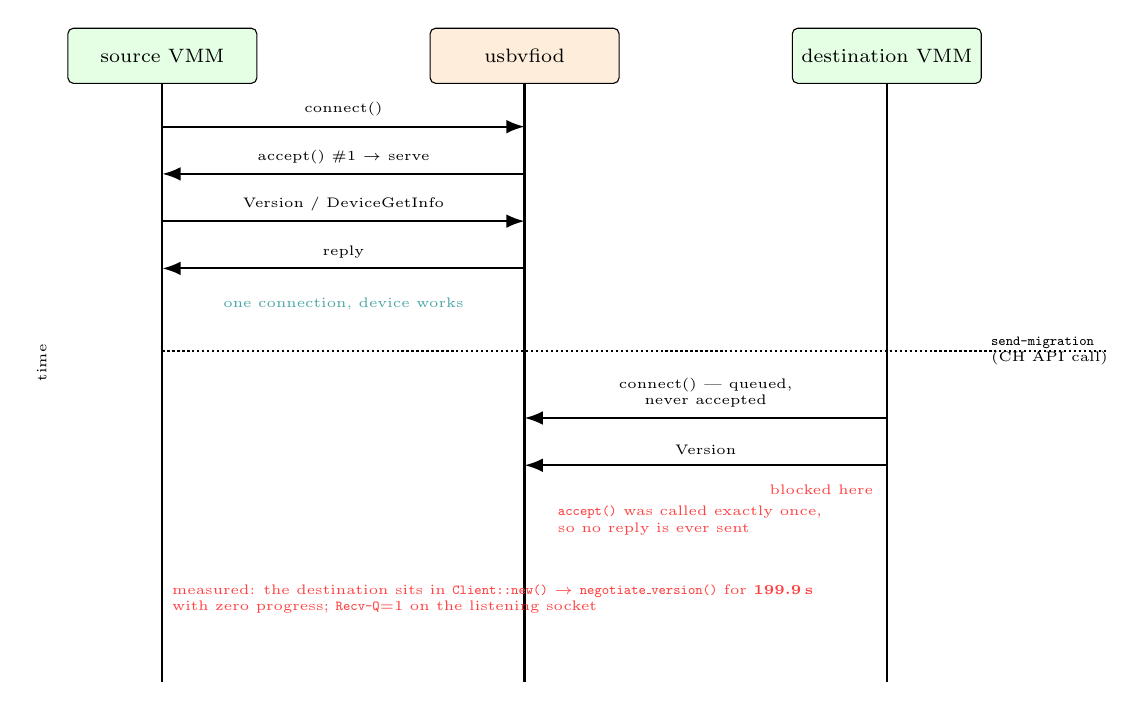
\begin{tikzpicture}[
  font=\scriptsize,
  >=Latex,
  x=1cm, y=1cm,
  ent/.style={draw, rounded corners=2pt, align=center, inner sep=3pt,
              minimum width=24mm, minimum height=7mm},
  msg/.style={->, thick},
]
  \node[ent, fill=green!10] (src) at (0,0) {source VMM};
  \node[ent, fill=orange!14] (uvf) at (4.6,0) {usbvfiod};
  \node[ent, fill=green!10] (dst) at (9.2,0) {destination VMM};

  \draw[thick] (src.south) -- ++(0,-7.6);
  \draw[thick] (uvf.south) -- ++(0,-7.6);
  \draw[thick] (dst.south) -- ++(0,-7.6);

  % time axis
  \node[font=\tiny, anchor=south, rotate=90] at (-1.35,-3.9) {time};

  % 1. the source is served normally
  \draw[msg] (0,-0.9) -- node[above, font=\tiny]{connect()} (4.6,-0.9);
  \draw[msg] (4.6,-1.5) -- node[above, font=\tiny]{accept() \#1 $\rightarrow$ serve} (0,-1.5);
  \draw[msg] (0,-2.1) -- node[above, font=\tiny]{Version / DeviceGetInfo} (4.6,-2.1);
  \draw[msg] (4.6,-2.7) -- node[above, font=\tiny]{reply} (0,-2.7);
  \node[font=\tiny, align=center, text=teal!70] at (2.3,-3.15)
       {one connection, device works};

  % 2. the migration is requested (a VMM-side API call, not a server message)
  \draw[thick, densely dotted] (0,-3.75) -- (12.0,-3.75);
  \node[font=\tiny, anchor=west, align=left] at (10.4,-3.75)
       {\texttt{send-migration}\\ \tiny (CH API call)};

  % 3. the destination connects and is never served
  \draw[msg] (9.2,-4.6) -- node[above, font=\tiny, align=center]{connect() --- queued,\\ never accepted} (4.6,-4.6);
  \draw[msg] (9.2,-5.2) -- node[above, font=\tiny]{Version} (4.6,-5.2);
  \node[red!75, font=\tiny, anchor=north east, align=right] at (9.15,-5.32)
       {blocked here};
  \node[font=\tiny, align=left, text=red!75, anchor=west] at (4.9,-5.9)
       {\texttt{accept()} was called exactly once,\\ so no reply is ever sent};

  % 4. measured outcome
  \node[font=\tiny, align=left, text=red!75, anchor=west] at (0,-6.9)
       {measured: the destination sits in \texttt{Client::new()} $\rightarrow$
        \texttt{negotiate\_version()} for \textbf{199.9\,s}\\ with zero progress;
        \texttt{Recv-Q}=1 on the listening socket};
\end{tikzpicture}

\caption{Measured deadlock of the unmodified stack. The vfio-user server calls
\code{accept()} exactly once, so the destination's connection is queued and its
version handshake is never answered; the migration never completes.}
\label{fig:deadlock}
\end{figure*}

\subsection{Root cause: one connection, one accept}
The server side of \code{vfio\_user}~0.1.5 serves a connection by calling
\code{listener.accept()} once and then looping over commands until the peer
closes. A second client therefore \emph{connects successfully} (the kernel
completes the handshake into the listen backlog) but is never served, which is
exactly the ``hangs forever'' symptom above. A cross-host migration would have
the same problem, and additionally the destination would have no device: the
guard for that exists only for kernel-VFIO devices
(\code{VFIO device does not support migration}), not for vfio-user.

\subsection{Device state would not transfer anyway}
Even with the hand-over solved, the vfio-user device contributes almost nothing
to a migration in this version. Its \code{Pausable}, \code{Transportable} and
\code{Migratable} implementations are empty, and its snapshot contains only the
generic PCI state (configuration space, INTx/MSI/MSI-X configuration and the
MSI-X table); device BAR state, opaque device state and DMA dirty tracking are
absent. There is no device-state region in the protocol implementation and no
parameter with which the destination could be pointed at a different vfio-user
server. This is why our design deliberately does \emph{not} try to move device
state: for a same-host migration the server process simply stays alive and keeps
the session, and only the \emph{client} that the server talks to changes.

%=====================================================================
\section{Design}
\label{sec:design}
%=====================================================================

\subsection{Goals and non-goals}
The goal is that a same-host live migration of a VM with a passed-through USB
storage device completes, and that the guest does not observe a device change.
Concretely we require: (i) the migration completes; (ii) the guest sees no
re-enumeration and no reset; (iii) data transferred across the migration is
neither lost nor duplicated; (iv) no change to the VMM beyond what is needed to
consume a fixed protocol crate. Non-goals are cross-host migration, USB classes
other than bulk storage, and isochronous transfers.

\subsection{Multi-client backend with a per-command lock}
The deadlock exists because the server serialises \emph{connections} even
though the commands it handles are mostly independent of the device. In the
crate, only \code{RegionRead}, \code{RegionWrite}, \code{DmaMap},
\code{DmaUnmap}, \code{SetIrqs} and \code{DeviceReset} invoke the backend;
\code{Version}, \code{DeviceGetInfo}, \code{DeviceGetRegionInfo} and
\code{GetIrqInfo} do not. Consequently a second client can complete its
handshake while the first is still attached, provided that the backend is
shared with a lock taken \emph{per command}.

Fig.~\ref{fig:multiclient} shows the resulting structure. A shared state object
owns the backend and the interrupt-ownership bookkeeping, and hands out one
handle per connection. Each handle implements the server backend trait by
delegating to the shared backend under a mutex for the duration of a single
call. The accept loop is replicated over a configurable number of threads, so
the process can serve the source and the destination simultaneously. The
default keeps the historical single-client behaviour unchanged, which matters
for the systemd integration where the server is expected to exit when its only
client goes away.

\begin{figure*}[t]
\centering
% Figure: multi-client backend design.
% Handshake commands never touch the backend, so a per-command lock lets the
% destination complete its handshake while the source is still connected.
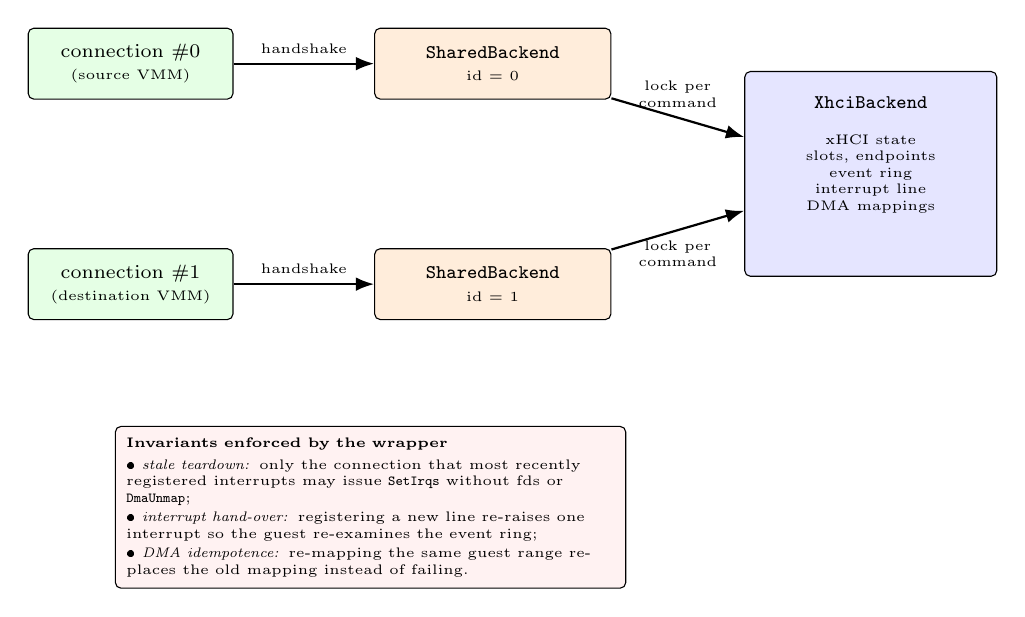
\begin{tikzpicture}[
  font=\scriptsize,
  >=Latex,
  node distance=8mm,
  blk/.style={draw, rounded corners=2pt, align=center, inner sep=4pt,
              minimum height=9mm},
  ar/.style={->, thick},
]
  % clients
  \node[blk, fill=green!10, minimum width=26mm] (c0) at (0,2.6)
        {connection \#0\\\tiny (source VMM)};
  \node[blk, fill=green!10, minimum width=26mm] (c1) at (0,-0.2)
        {connection \#1\\\tiny (destination VMM)};

  % handles
  \node[blk, fill=orange!14, minimum width=30mm] (h0) at (4.6,2.6)
        {\texttt{SharedBackend}\\\tiny id = 0};
  \node[blk, fill=orange!14, minimum width=30mm] (h1) at (4.6,-0.2)
        {\texttt{SharedBackend}\\\tiny id = 1};

  % backend
  \node[blk, fill=blue!10, minimum width=32mm, minimum height=26mm] (be) at (9.4,1.2) {};
  \node[font=\scriptsize\bfseries] at (9.4,2.1) {\texttt{XhciBackend}};
  \node[font=\tiny, align=center] at (9.4,1.2)
        {xHCI state\\slots, endpoints\\event ring\\interrupt line\\DMA mappings};

  \draw[ar] (c0) -- node[above, font=\tiny]{handshake} (h0);
  \draw[ar] (c1) -- node[above, font=\tiny]{handshake} (h1);
  \draw[ar] (h0) -- node[above, font=\tiny, align=center]{lock per\\command} (be);
  \draw[ar] (h1) -- node[below, font=\tiny, align=center]{lock per\\command} (be);

  % invariant box
  \node[draw, rounded corners=2pt, fill=red!5, align=left, inner sep=4pt,
        font=\tiny, text width=62mm, anchor=north west] at (-0.2,-2.0)
  {\textbf{Invariants enforced by the wrapper}\\[2pt]
   \textbullet\ \emph{stale teardown:} only the connection that most recently
     registered interrupts may issue \texttt{SetIrqs} without fds or
     \texttt{DmaUnmap};\\[1pt]
   \textbullet\ \emph{interrupt hand-over:} registering a new line re-raises one
     interrupt so the guest re-examines the event ring;\\[1pt]
   \textbullet\ \emph{DMA idempotence:} re-mapping the same guest range replaces
     the old mapping instead of failing.};
\end{tikzpicture}

\caption{Multi-client backend. Handshake commands never take the lock, so the
destination VMM can connect while the source is still attached; the device
state itself lives in the shared backend and therefore survives the hand-over.}
\label{fig:multiclient}
\end{figure*}

\subsection{Ownership: a departing client must not tear the device down}
\label{sec:ownership}
Allowing two clients exposes a hazard that a single-client server never had.
When the migration completes, the \emph{source} VMM shuts its device down and
sends two destructive commands: \code{SetIrqs} with an empty descriptor list
(disable interrupts) and \code{DmaUnmap} for the regions it mapped. Both arrive
\emph{after} the destination has already registered its own interrupts and DMA
mappings, and both would be applied to the shared backend. The result we
measured is severe: the destination is left with a dummy interrupt line, no
completion is ever signalled, and the guest concludes that the controller is
dead and aborts the running I/O.

The wrapper therefore tracks which connection most recently registered
interrupts and lets only that connection issue the destructive counterparts.
Teardown from any other connection is logged and ignored. This is deliberately
coarse: it is correct for the hand-over case, which is the case that needs it,
and it cannot be triggered accidentally by the active client.

\subsection{Interrupt hand-over correctness}
\label{sec:interrupt}
A subtler, timing-dependent defect remains even after
Section~\ref{sec:ownership}. The interrupter signals every event by writing to
the currently installed interrupt line. During a hand-over there is a window in
which a transfer may complete \emph{before} the destination's line is
installed: the completion event is written into the guest's event ring (which
is in guest memory and therefore already correct), but the interrupt is
delivered to the event descriptor of the VMM that is exiting. The event is
then never noticed: the guest does not re-read its event ring without an
interrupt, the copy stalls, and---because the USB stack eventually tries to
recover---the guest starts issuing device resets that the emulated controller
correctly rejects as a context state error.

Our fix is to re-raise one interrupt immediately after a new line is installed.
A spurious MSI-X interrupt is harmless: the guest inspects the event ring,
finds the pending completion (or nothing) and continues. This converts a lost
interrupt into at most one redundant ring scan.

\subsection{DMA mapping idempotence}
\label{sec:dma}
Because source and destination map the \emph{same} guest memory under
\code{memory\_mode=memfds}, the destination re-issues \code{DmaMap} for ranges
that the source already mapped. A naive ``insert only'' bus rejects the
duplicate as an overlap. We make the DMA bus replace a mapping that starts at
the same address, while still rejecting a genuine overlap at a different
address, and we make a failed insert leave the bus untouched. We also implement
the unmap path, which the VMM invokes when it destroys a device and which was
previously unimplemented.

%=====================================================================
\section{Implementation}
\label{sec:implementation}
%=====================================================================

\subsection{usbvfiod}
The change is confined to six files (about 380 added and 30 removed lines):
a new \code{shared\_backend} module implementing the wrapper and the ownership
rules; the accept-loop and lifecycle logic in \code{main}; a
\code{-{}-max-clients} option; the idempotent DMA bus; and the DMA, reset and
interrupt-registration paths of the xHCI backend. The device emulation itself
is untouched. Unit tests were extended from 109 to 112, and the project's
strict lint configuration (\code{clippy} with all, nursery and cargo groups
denied) passes.

\subsection{Protocol crate}
One behavioural bug in \code{vfio\_user}~0.1.5 had to be fixed for the reset
semantics to be sane. The client parses the device's reset capability by
comparing the masked flag word with \emph{inequality}, which inverts the result:
a server that advertises ``not resettable'' is reported as resettable, so the
VMM issues a device reset on every connection---including once per connection
during a migration. The fix is a one-line equality comparison. Because the
crate is consumed by the VMM, the fix is applied to the VMM's dependency graph
rather than to \code{usbvfiod}, which only uses the server side.

\subsection{Cloud Hypervisor integration}
No CH code was modified. The only integration artefact is a
\code{[patch.crates-io]} entry that points CH at the fixed crate. Because the
crate lives in a monorepo whose manifest also references a sibling
\code{vfio-bindings} crate that has diverged from the published version, the
patch deliberately uses a variant of the fix branch in which that crate resolves
from crates.io; otherwise two copies of \code{vfio-bindings} coexist and their
types no longer unify. This is a build-level detail, not a design change, and it
is documented so that it can be dropped once the fix is released upstream.

\subsection{Guest image and measurement harness}
Measurement honesty turned out to require as much care as the device code, and
we record the decisions because they changed our verdict twice.

\emph{Guest image.} The Ubuntu live-server ISO cannot be booted directly: its
initrd insists on finding a live medium and ignores \code{root=}, and the
minimal squashfs ships an empty \code{/lib/modules}, so \code{usb-storage}
cannot be loaded after the switch. We therefore unpack the ISO, graft the
module tree out of the initrd, rebuild the initrd without the casper hooks and
pack a bootable ext4 image. exfat, which real sticks use, lives in
\code{linux-modules-extra} and is merged in explicitly.

\emph{Console capture.} CH opens a serial \code{file=} target with
\code{File::create()}, so the destination VMM truncates the log when it starts;
the pre-migration evidence disappears exactly when it becomes interesting. We
capture the console through a FIFO kept open by a reader that never sees EOF.

\emph{Verdict source.} The migration also re-creates the destination's serial
device, which resets the guest TTY. Progress written only to the console then
looks like a hang although the guest is fine. We therefore make the guest log
to a file and treat the serial console as a best-effort mirror, and we compute
the verdict from the guest's own log after stopping the VMs and mounting the
disk image---with the journal replayed, because a read-only \code{noload} mount
hides the most recent writes. A guest heartbeat service, finally, distinguishes
``guest frozen'' from ``console broken''.

%=====================================================================
\section{Evaluation}
\label{sec:evaluation}
%=====================================================================

\subsection{Methodology}
The workload is a 128\,MiB file copied from the passed-through stick to the
guest's own disk with \code{dd}, in a systemd unit that starts at boot. The
harness waits until the guest reports that the copy has begun, waits a further
four seconds so that the transfer is in flight, and then migrates the VM. A run
is successful only if all four of the following hold: the copy window strictly
contains the migration instant; the md5 of the copied file equals the md5 of
the source file on the stick; the guest shows no enumeration after boot; and no
reset or I/O error appears. The md5 comparison is made inside the guest
against the stick itself, so it also verifies that the device remained readable
after the migration. We ran the experiment 10 times after the fixes described in
Section~\ref{sec:design} were in place.

\subsection{Results}
All 10 runs pass. Table~\ref{tab:results} lists the per-run figures;
Fig.~\ref{fig:downtime} shows the downtime distribution. Downtime is measured
by CH (\code{downtime\_ms}), not by the harness. Copy duration is the time the
guest takes to copy the file, which is chosen to be long enough that the
migration necessarily falls inside the copy window; the variation is dominated
by USB~2.0 read throughput and by page-cache effects, not by the migration.

\begin{table}[t]
\centering
\caption{Acceptance runs (post-fix). ``Spans'' means the copy window contains
the migration instant; ``enums'' counts guest enumerations after boot.}
\label{tab:results}
\footnotesize
\setlength{\tabcolsep}{4pt}
\begin{tabular}{@{}rrrrl@{}}
\toprule
Run & Downtime (ms) & Copy (s) & Spans & md5 / enums \\
\midrule
1  & 17 & 20.6 & yes & match / 0 \\
2  & 18 & 30.2 & yes & match / 0 \\
3  & 15 & 33.9 & yes & match / 0 \\
4  & 17 & 33.5 & yes & match / 0 \\
5  & 15 & 35.3 & yes & match / 0 \\
6  & 16 & 32.4 & yes & match / 0 \\
7  &  4 & 28.4 & yes & match / 0 \\
8  &  4 & 13.2 & yes & match / 0 \\
9  &  6 & 15.0 & yes & match / 0 \\
10 & 17 & 52.4 & yes & match / 0 \\
\midrule
\multicolumn{2}{@{}l}{median downtime} & \multicolumn{2}{l}{15.5\,ms} & \\
\multicolumn{2}{@{}l}{target} & \multicolumn{2}{l}{$\le 2000$\,ms} & \\
\bottomrule
\end{tabular}
\end{table}

\begin{figure}[t]
\centering
% Figure: measured live-migration downtime for the ten acceptance runs.
% Columns of data/runs.dat: run index, downtime (ms), copy duration (s).
\begin{tikzpicture}
\begin{axis}[
  width=\columnwidth, height=4.6cm,
  ybar, bar width=6pt,
  xlabel={run},
  ylabel={downtime (ms)},
  xmin=0.4, xmax=10.6, ymin=0, ymax=20,
  xtick=data,
  grid=major, grid style={gray!22},
  tick label style={font=\scriptsize},
  label style={font=\scriptsize},
  nodes near coords, nodes near coords style={font=\tiny},
  every node near coord/.append style={yshift=1pt},
]
  \addplot[fill=blue!35, draw=blue!60!black] table[x index=0, y index=1]
    {data/runs.dat};
\end{axis}
\end{tikzpicture}

\caption{Measured downtime of the ten acceptance runs. The goal of
$\le 2000$\,ms is far above the plotted range.}
\label{fig:downtime}
\end{figure}

\subsection{Timeline of a representative run}
Fig.~\ref{fig:copy} shows the guest's copy progress for one run together with
the migration instant. The copy is visibly interrupted in the sense that the
curve is not perfectly smooth, but it continues across the migration and
finishes with $rc=0$; the guest never restarts the transfer. The final
throughput in this run was $5.7$\,MB/s ($5.4$\,MiB/s), consistent with the stick's USB~2.0
read performance measured outside the migration.

\begin{figure}[t]
\centering
% Figure: guest copy progress in the representative run (real measurement).
% Columns of data/copy_progress.dat: seconds since copy start, MiB copied.
\begin{tikzpicture}
\begin{axis}[
  width=\columnwidth, height=5.0cm,
  xlabel={time since copy start (s)},
  ylabel={copied (MiB)},
  xmin=0, xmax=26, ymin=0, ymax=140,
  grid=major, grid style={gray!22},
  tick label style={font=\scriptsize},
  label style={font=\scriptsize},
  legend style={font=\tiny, at={(0.02,0.98)}, anchor=north west, draw=gray!40,
                fill=white, fill opacity=0.85, text opacity=1},
]
  \addplot[very thick, blue!70!black] table[x index=0, y index=1]
    {data/copy_progress.dat};
  \addlegendentry{guest \texttt{dd} progress}
  \addplot[red, dashed, very thick, domain=0:26] {0};
  \addlegendentry{migration at $t=7.39$\,s}
  \draw[red, dashed, very thick] (axis cs:7.393,0) -- (axis cs:7.393,140);
  \addplot[only marks, mark=*, mark size=1.8pt, red] coordinates {(7.393,19)};
\end{axis}
\end{tikzpicture}

\caption{Guest copy progress in the representative run (128\,MiB). The
migration occurs at $t=7.39$\,s, inside the copy window; the copy completes at
$t=23.54$\,s with status 0.}
\label{fig:copy}
\end{figure}

\subsection{Data-path continuity under the hand-over}
Fig.~\ref{fig:rate} compares the USB transaction rate across the hand-over
before and after the interrupt fix, both taken from the vfio-user server's
packet capture. Before the fix the rate drops to zero at the hand-over and
stays there: the device is still powered and the server still holds it, but no
further transfer is initiated because the guest is waiting for a completion it
was never told about. After the fix the rate continues across the hand-over and
only falls to zero when the copy has finished. This figure is the clearest
evidence that the failures we saw were a lost-notification problem rather than
a transport or device problem.

\begin{figure}[t]
\centering
% Figure: USB transfer rate across the hand-over (real pcap measurements).
% Columns: seconds since copy start, packets per second.
\begin{tikzpicture}
\begin{axis}[
  width=\columnwidth, height=5.0cm,
  xlabel={time since copy start (s)},
  ylabel={USB packets/s},
  xmin=-6, xmax=32, ymin=0, ymax=2250,
  grid=major, grid style={gray!22},
  tick label style={font=\scriptsize},
  label style={font=\scriptsize},
  legend style={font=\tiny, at={(0.02,0.98)}, anchor=north west, draw=gray!40,
                fill=white, fill opacity=0.85, text opacity=1},
]
  \addplot[very thick, blue!70!black] table[x index=0, y index=1]
    {data/rate_success.dat};
  \addlegendentry{after the fix: transfers continue}
  \addplot[very thick, red!70!black] table[x index=0, y index=1]
    {data/rate_failure.dat};
  \addlegendentry{before the fix: stalls at the hand-over}
  \draw[black, dashed, thick] (axis cs:7.393,0) -- (axis cs:7.393,2250);
  \node[font=\tiny, anchor=north east, rotate=90] at (axis cs:7.0,2200) {hand-over};
\end{axis}
\end{tikzpicture}

\caption{USB transaction rate across the hand-over, measured at the vfio-user
server. Without the interrupt fix, transfers stop at the hand-over and never
resume; with the fix they continue until the copy completes.}
\label{fig:rate}
\end{figure}

\subsection{Defects found}
Table~\ref{tab:defects} summarises the three defects that had to be fixed. The
first two are deterministic and reproduce on every run; the third is
timing-dependent and appeared in roughly one run in five before it was fixed.

\begin{table}[t]
\centering
\caption{Defects found and fixed.}
\label{tab:defects}
\footnotesize
\setlength{\tabcolsep}{3pt}
\begin{tabular}{@{}p{1.45cm}p{2.1cm}p{3.1cm}@{}}
\toprule
Defect & Symptom & Fix \\
\midrule
single-accept server & destination blocks 199.9\,s in the handshake & per-command lock, multi-client accept \\
stale teardown & guest declares controller dead after migration & interrupt-ownership rule \\
lost hand-over interrupt & copy stalls with no error (intermittent) & re-raise one interrupt on registration \\
\bottomrule
\end{tabular}
\end{table}

\subsection{Discussion of the measurements}
Two points about the method are worth stating explicitly, because both changed
our conclusions during the work. First, host-side observation is not
sufficient: the packet capture and the VMM logs looked healthy in a run whose
guest had in fact stopped making progress. Second, a single passing run is not
evidence for a timing-dependent fix: the defect in Section~\ref{sec:interrupt}
passed four consecutive runs before it failed on the fifth, and only repeated
runs after the fix justify the claim of 10 out of 10.

%=====================================================================
\section{Discussion and Limitations}
\label{sec:discussion}
%=====================================================================

\paragraph{What is transparent.}
At the USB level the guest is undisturbed: it enumerates the device once, at
boot, and never again; it observes no reset, no port status change and no I/O
error; the file it copies is byte-identical to the source. This is the property
that matters for storage passthrough and it is the one we set out to obtain.

\paragraph{What is not.}
One guest-visible disturbance remains and we do not want to hide it: after the
migration the guest reprints its login banner. The destination re-creates the
serial device, which resets the guest TTY. This is a property of the VMM's
serial device model, not of the USB path, and it does not affect the device. We
report it because a claim of ``zero perception'' should be stated at the
granularity at which it is true.

\paragraph{No explicit quiesce.}
We did not implement a bounded drain of in-flight transfers before the
hand-over. Transfers that are in flight when the migration happens are handled
by the re-raise mechanism plus the guest's own retry logic; the guest may
therefore in principle have to retry a command, although in our runs the
completion arrived through the re-raise and the copy was not restarted. A
production implementation would add an explicit quiesce to bound this, and a
guest-cooperative handshake if the downtime budget were tighter.

\paragraph{Scope.}
The evaluation covers bulk storage on a USB~2.0 stick, one device per
controller, Linux guests, and same-host migration. Other classes (HID,
isochronous audio, serial) have different in-flight semantics; isochronous
traffic in particular cannot be made lossless by retrying and is not supported
by the underlying \code{nusb} library. Cross-host migration is a different
problem: it needs the device state to be transferred or an equivalent device to
be provided on the destination, and it cannot preserve a host-side session.

\paragraph{Process lifecycle.}
With more than one client the server no longer exits when the last client
disconnects, which is a deliberate change needed for the hand-over. Deployments
that rely on exit-on-disconnect (for example socket-activated systemd units)
must either keep the default single-client mode or manage the process
explicitly.

%=====================================================================
\section{Conclusion and Future Work}
\label{sec:conclusion}
%=====================================================================

We set out to make a USB storage device survive a live migration of the VM it
is passed through to, and we found that the path did not merely fail---it
deadlocked, because a vfio-user server built for one client cannot serve the
destination while the source is still attached. The fix follows from a
property of the protocol that is easy to miss: the handshake does not touch the
device, so the device lock does not have to be held for the lifetime of a
connection. On top of that, two further defects had to be fixed before the
hand-over was correct rather than merely possible: ownership of destructive
teardown, and the synchronisation of the interrupt line across the hand-over.
With those in place, a 128\,MiB copy that spans the migration completes in 10
out of 10 runs with 4--18\,ms of downtime and byte-identical data.

Future work falls into three groups. First, an explicit quiesce and a
guest-cooperative protocol would make in-flight behaviour deterministic instead
of relying on retry. Second, a protocol-level device-state region would allow
the device to be reconstructed on another host, which is the prerequisite for
cross-host migration; our measurements show that the current protocol carries
none of the required state. Third, the same technique should be evaluated for
other device classes and for multiple devices on one controller, where the
ownership rules we introduced would need to become per-device.

%=====================================================================
\appendices
\section{Reproduction}
%=====================================================================

The full harness, the development log and the raw measurement data are part of
the accompanying artefact. In outline:

\begin{enumerate}
  \item build the guest image: \code{guest/build-guest.sh};
  \item place a 128\,MiB \code{testfile.bin} on the stick and record its md5 in
        \code{guest/testfile.md5};
  \item run \code{guest/usb-migration-demo.sh} (add \code{PAUSE=1} for a
        step-by-step narrated run);
  \item read the verdict, which is derived from the guest's own log as
        described in Section~\ref{sec:implementation}.
\end{enumerate}

\begin{thebibliography}{99}
\footnotesize

\bibitem{clark2005live}
C.~Clark, K.~Fraser, S.~Hand, J.~G. Hansen, E.~Jul, C.~Limpach, I.~Pratt, and
A.~Warfield, ``Live migration of virtual machines,'' in \emph{Proc. 2nd USENIX
Symp. Networked Systems Design and Implementation (NSDI)}, 2005.
[Online]. Available: \url{https://www.usenix.org/conference/nsdi-05/live-migration-virtual-machines}

\bibitem{kivity2007kvm}
A.~Kivity, Y.~Kamay, D.~Laor, U.~Lublin, and A.~Liguori, ``kvm: the Linux
virtual machine monitor,'' in \emph{Proc. Linux Symposium}, vol.~1, 2007,
pp.~225--230. [Online]. Available:
\url{https://www.kernel.org/doc/ols/2007/ols2007v1-pages-225-230.pdf}

\bibitem{agache2020firecracker}
A.~Agache, M.~Brooker, A.~Iordache, A.~Liguori, R.~Neugebauer, P.~Piwonka, and
D.-M. Popa, ``Firecracker: lightweight virtualization for serverless
applications,'' in \emph{Proc. 17th USENIX Symp. Networked Systems Design and
Implementation (NSDI)}, 2020. [Online]. Available:
\url{https://www.usenix.org/conference/nsdi20/presentation/agache}

\bibitem{hirofuchi2005usbip}
T.~Hirofuchi, E.~Kawai, K.~Fujikawa, and H.~Sunahara, ``USB/IP: a transparent
device sharing technology over IP network,'' \emph{IPSJ Digital Courier},
vol.~1, 2005, doi: 10.2197/ipsjdc.1.394. [Online]. Available:
\url{https://www.jstage.jst.go.jp/article/ipsjdc/1/0/1_0_394/_article}

\bibitem{qemuvfiouser}
QEMU, ``vfio-user protocol specification.'' [Online]. Available:
\url{https://www.qemu.org/docs/master/interop/vfio-user.html}

\bibitem{chvfiouser}
Cloud Hypervisor, ``VFIO-user HOWTO (docs/vfio-user.md).'' [Online]. Available:
\url{https://github.com/cloud-hypervisor/cloud-hypervisor/blob/main/docs/vfio-user.md}

\bibitem{chlive}
Cloud Hypervisor, ``Live migration (docs/live\_migration.md).'' [Online].
Available:
\url{https://github.com/cloud-hypervisor/cloud-hypervisor/blob/main/docs/live_migration.md}

\bibitem{chrepo}
Cloud Hypervisor, ``A virtual machine monitor for modern cloud workloads.''
[Online]. Available: \url{https://github.com/cloud-hypervisor/cloud-hypervisor}

\bibitem{kernelvfio}
The Linux Kernel documentation, ``VFIO --- virtual function I/O.'' [Online].
Available: \url{https://docs.kernel.org/driver-api/vfio.html}

\bibitem{kernelusbip}
The Linux Kernel documentation, ``USB/IP protocol.'' [Online]. Available:
\url{https://docs.kernel.org/usb/usbip_protocol.html}

\bibitem{kernelusb}
The Linux Kernel documentation, ``USB support.'' [Online]. Available:
\url{https://docs.kernel.org/usb/index.html}

\bibitem{qemuusb}
QEMU, ``USB emulation.'' [Online]. Available:
\url{https://www.qemu.org/docs/master/system/devices/usb.html}

\bibitem{virtio12}
OASIS, ``Virtual I/O device (VIRTIO) version 1.2,'' 2022. [Online]. Available:
\url{https://docs.oasis-open.org/virtio/virtio/v1.2/virtio-v1.2.html}

\bibitem{xhcispec}
Intel Corporation, ``eXtensible host controller interface for universal serial
bus (xHCI) specification, revision 1.2.'' [Online]. Available:
\url{https://www.intel.com/content/dam/www/public/us/en/documents/technical-specifications/extensible-host-controler-interface-usb-xhci.pdf}

\bibitem{usbbot}
USB Implementers Forum, ``Universal serial bus mass storage class bulk-only
transport, revision 1.0,'' 1999. [Online]. Available:
\url{https://www.usb.org/sites/default/files/usbmassbulk_10.pdf}

\bibitem{rustvmmvfio}
rust-vmm, ``rust-vmm/vfio.'' [Online]. Available:
\url{https://github.com/rust-vmm/vfio}

\bibitem{vfiousercrate}
``vfio\_user 0.1.5 --- Rust crate documentation.'' [Online]. Available:
\url{https://docs.rs/vfio_user/0.1.5}

\bibitem{nusb}
K.~Mehall, ``nusb: a new pure-Rust library for cross-platform low-level USB.''
[Online]. Available: \url{https://github.com/kevinmehall/nusb}

\bibitem{usbvfiodrepo}
Cyberus Technology, ``usbvfiod: a vfio-user server for USB pass-through.''
[Online]. Available: \url{https://github.com/cyberus-technology/usbvfiod}

\bibitem{libvfiouser}
Nutanix, ``libvfio-user: framework for emulating devices in userspace.''
[Online]. Available: \url{https://github.com/nutanix/libvfio-user}

\bibitem{memfd}
Linux man-pages, ``memfd\_create(2).'' [Online]. Available:
\url{https://man7.org/linux/man-pages/man2/memfd_create.2.html}

\end{thebibliography}

\end{document}
